% ============================================================
%  Diseño, Análisis y Optimización mediante Machine Learning
%  de una Estribera de Motocicleta de Trial
%  Autor: Antonio Vital Juncar
% ============================================================
\documentclass[11pt, a4paper]{article}

\usepackage[utf8]{inputenc}
\usepackage[T1]{fontenc}
\usepackage[spanish]{babel}
\usepackage[top=2.2cm, bottom=2.2cm, left=2.4cm, right=2.4cm]{geometry}
\usepackage{graphicx}
\usepackage{booktabs}
\usepackage{float}
\usepackage{caption}
\usepackage{amsmath}
\usepackage{parskip}
\usepackage{microtype}
\usepackage{lmodern}
\usepackage{fancyhdr}
\usepackage{titlesec}
\usepackage{enumitem}
\usepackage{xcolor}
\usepackage[hidelinks]{hyperref}
\usepackage{tikz}
\usepackage[most]{tcolorbox}
\usepackage{multirow}
\usepackage{array}
\usetikzlibrary{shapes.rounded, arrows.meta, positioning, fit}

% Paleta de colores
\definecolor{nasa}{RGB}{11,61,145}
\definecolor{verde}{RGB}{39,174,96}
\definecolor{rojo}{RGB}{192,57,43}
\definecolor{naranja}{RGB}{243,156,18}
\definecolor{gris}{RGB}{100,100,100}
\definecolor{azulclaro}{RGB}{220,230,245}
\definecolor{verdeclaro}{RGB}{220,245,230}

% Formato de secciones
\titleformat{\section}
  {\large\bfseries\color{nasa}}{\thesection.}{0.5em}{}
  [\vspace{-4pt}\textcolor{nasa!40}{\rule{\linewidth}{0.6pt}}\vspace{3pt}]
\titleformat{\subsection}
  {\normalsize\bfseries\color{gris}}{\thesubsection.}{0.4em}{}

% Cabecera y pie
\pagestyle{fancy}\fancyhf{}
\fancyhead[L]{\small\color{nasa}\textbf{Estribera de Trial - CAD, FEM, CAM \& ML}}
\fancyhead[R]{\small\color{gris}Antonio Vital Juncar}
\fancyfoot[C]{\small\thepage}
\renewcommand{\headrulewidth}{0.4pt}

\hypersetup{colorlinks=true, linkcolor=nasa, urlcolor=nasa,
  pdftitle={Diseno y Optimizacion ML Estribera de Trial}}

\graphicspath{{figures/}}

% Macro para imágenes de usuario
% graphicspath ya apunta a figures/, basta con el nombre de archivo
\newcommand{\imagenph}[2]{%
  \includegraphics[width=#2]{#1}%
}

% ─────────────────────────────────────────────────────────────────────────────
\begin{document}

% ============================================================
%  PORTADA
% ============================================================
\begin{titlepage}
\centering
\vspace*{0.2cm}

{\color{nasa}\rule{\linewidth}{1.5pt}}\\[0.4em]
{\Huge\bfseries\color{nasa}
  Diseño y Optimización de una\\[0.3em]
  Estribera de Trial\\[0.3em]
  mediante Machine Learning}\\[0.3em]
{\color{nasa}\rule{\linewidth}{1.5pt}}\\[0.6em]

{\Large\itshape\color{gris}
  Estudio integral CAD $\cdot$ FEM $\cdot$ CAM $\cdot$ ML
  -- Aluminio 7075-T6}\\[0.8em]

\imagenph{fig_01_render_isometrico.png}{0.40\textwidth}\\[0.8em]

\bgroup
\def\arraystretch{1.15}
\begin{tabular}{@{} l l @{}}
  \toprule
  \multicolumn{2}{c}{\Large\textbf{Resumen del Proyecto}}\\[0.4em]
  \midrule
  \textbf{Pieza}               & Estribera de motocicleta de trial (mecanizada) \\
  \textbf{Material}            & Aluminio 7075-T6 $\cdot$ $R_{p0{,}2}=503$ MPa \\
  \textbf{Carga FEM}           & 2\,000 N sobre superficie de dientes \\
  \textbf{Dataset}             & 27 variantes (diseño factorial $3\times3\times3$) \\
  \textbf{Modelo seleccionado} & \textbf{\color{verde}Gradient Boosting} \\
  \textbf{R$^{2}$ global}      & \textbf{\color{verde}0{,}9531}
                                 \textit{(validación cruzada 5 iteraciones)} \\
  \textbf{Von Mises - diseño óptimo}
                               & \textbf{\color{verde}241{,}6 MPa}
                                 \textit{(límite: 335{,}3 MPa, FS\,=\,1{,}5)} \\
  \textbf{Entorno}             & Python / Jupyter Notebook \\
  \bottomrule
\end{tabular}
\egroup

\vfill

{\Large\bfseries Antonio Vital Juncar}\\[0.3em]
{\large\color{gris}2026}

\vspace{0.5em}

{\footnotesize\color{gris}
  Software utilizado: FreeCAD (CAD, FEM, CAM y planos) $\cdot$ Python 3.10 (machine learning).
}
\end{titlepage}
% ============================================================

\tableofcontents
\newpage

% ============================================================
\section{Resumen del proyecto}
% ============================================================

Este proyecto demuestra la integración de cuatro disciplinas de ingeniería y ciencia
de datos: diseño asistido por ordenador (CAD), análisis de elementos finitos (FEM),
fabricación asistida por ordenador (CAM) y aprendizaje automático (ML). Todas ellas
se aplican a un caso de uso real: la optimización de una estribera de motocicleta de trial.

El flujo de trabajo va desde el modelado paramétrico de la pieza hasta la evaluación
económica de su fabricación, pasando por la simulación estructural y la generación de
un modelo predictivo capaz de evaluar nuevas combinaciones geométricas sin necesidad
de realizar simulaciones adicionales.

% Flujo de trabajo
\subsection{Flujo de trabajo}

\begin{center}
\resizebox{\linewidth}{!}{%
\begin{tikzpicture}[
  nodo/.style={
    rounded corners=4pt, draw=nasa, fill=azulclaro,
    text width=2.0cm, align=center, minimum height=1.0cm,
    font=\small\bfseries\color{nasa}
  },
  flecha/.style={-Stealth, thick, color=nasa}
]
  \node[nodo] (cad) {CAD\\FreeCAD\\Paramétrico};
  \node[nodo] (fem)  [right=0.9cm of cad]  {FEM\\27 variantes\\estáticas};
  \node[nodo] (cam)  [right=0.9cm of fem]  {CAM\\Tiempos de\\mecanizado};
  \node[nodo] (eco)  [right=0.9cm of cam]  {Estudio\\Económico\\Costes};
  \node[nodo] (ds)   [right=0.9cm of eco]  {Dataset\\27 filas\\$\times$\,5 targets};
  \node[nodo,fill=verdeclaro,draw=verde] (ml) [right=0.9cm of ds]
    {ML\\Gradient\\Boosting};

  \draw[flecha] (cad) -- (fem);
  \draw[flecha] (fem) -- (cam);
  \draw[flecha] (cam) -- (eco);
  \draw[flecha] (eco) -- (ds);
  \draw[flecha] (ds)  -- (ml);

  \node[below=0.5cm of cad,  font=\footnotesize\color{gris}] {3 vars $\times$ 3 niveles};
  \node[below=0.5cm of fem,  font=\footnotesize\color{gris}] {2\,000 N, M10};
  \node[below=0.5cm of cam,  font=\footnotesize\color{gris}] {CNC 3 ejes};
  \node[below=0.5cm of eco,  font=\footnotesize\color{gris}] {Material + operac.};
  \node[below=0.5cm of ds,   font=\footnotesize\color{gris}] {3 features, 5 targets};
  \node[below=0.5cm of ml,   font=\footnotesize\color{verde}] {R$^2$\,=\,0{,}953};
\end{tikzpicture}%
}
\end{center}

% Resultados clave
\subsection{Resultados clave}

\begin{tcolorbox}[
  colback=azulclaro, colframe=nasa, arc=4pt,
  title={\bfseries\color{white} Resultados del modelo ML (Gradient Boosting, evaluación sobre conjunto de prueba — holdout 20\,\%)},
  fonttitle=\small
]
\begin{center}
\small
\begin{tabular}{lcccc}
  \toprule
  \textbf{Variable objetivo} & \textbf{MAE} & \textbf{RMSE} & \textbf{R$^{2}$} & \textbf{Unidad}\\
  \midrule
  Masa                     & 0{,}428 & 0{,}559 & \color{verde}\textbf{0{,}9948} & g     \\
  Tensión Von Mises (máx.) & 14{,}68 & 16{,}34 & \color{naranja}\textbf{0{,}754}  & MPa   \\
  Deformación máx.         & 0{,}031 & 0{,}039 & \color{verde}\textbf{0{,}9774} & mm    \\
  Tiempo total CNC         & 0{,}035 & 0{,}044 & \color{verde}\textbf{0{,}9996} & min   \\
  Coste total CNC          & 0{,}071 & 0{,}078 & \color{verde}\textbf{0{,}9957} & EUR   \\
  \midrule
  \textbf{Global (media)}  &  {-}    &  {-}    & \color{verde}\textbf{0{,}944}  & {-}   \\
  \bottomrule
\end{tabular}
\end{center}
\end{tcolorbox}

\begin{tcolorbox}[
  colback=verdeclaro, colframe=verde, arc=4pt,
  title={\bfseries\color{white} Diseño óptimo identificado por el modelo},
  fonttitle=\small
]
\small
Combinación con mejor balance tensión-coste-masa (de 216 evaluadas):
\textbf{Largo\,=\,60\,mm, Altura\,=\,14\,mm, Nervio\,=\,12\,mm}.
Tensión Von Mises predicha: \textbf{\color{verde}241{,}6\,MPa}
(límite admisible: 335{,}3\,MPa; margen resistente residual: 28\,\%).
Coste CNC predicho: \textbf{12{,}49\,EUR}. Masa: \textbf{100{,}23\,g}.
\end{tcolorbox}

% Qué se hizo en cada etapa
\subsection{Qué se hizo en cada etapa}

\begin{enumerate}[leftmargin=1.6cm, label=\textbf{\arabic*.}]
  \item \textbf{Diseño paramétrico (CAD):} Modelado de la estribera en FreeCAD con tres
    variables de diseño (Largo, Altura y Nervio), cada una con tres valores posibles,
    generando un diseño factorial completo de $3^3=27$ variantes y sus correspondientes
    planos técnicos.
  \item \textbf{Análisis FEM:} Ensayo estático de las 27 variantes con una carga de
    2\,000\,N sobre la superficie de los dientes y condiciones de contorno fijas por
    tornillo M10 y tope estructural. Se extrajo la tensión Von Mises máxima y la
    deformación máxima de cada variante.
  \item \textbf{Fabricación asistida (CAM):} Simulación de las estrategias de mecanizado
    CNC de 3 ejes para cada variante, estimando los tiempos de ciclo reales con un
    factor de penalización de 1{,}25.
  \item \textbf{Estudio económico:} Cálculo del coste de fabricación en función del
    material consumido y del tiempo de mecanizado.
  \item \textbf{Machine learning:} Entrenamiento de cinco modelos de regresión y
    selección del mejor. Se genera una función de predicción que evalúa nuevas
    parametrizaciones sin necesidad de simulación adicional.
\end{enumerate}


% ============================================================
\section{Configuración del estudio}
% ============================================================

\subsection{La pieza: estribera de motocicleta de trial}

La \textit{estribera} es el elemento sobre el que el piloto apoya el pie durante la
conducción. En el \textit{trial}, competición técnica de habilidad sobre obstáculos
naturales o artificiales, la estribera está sometida a cargas de impacto y a requisitos
de ligereza más exigentes que en disciplinas convencionales.

\begin{figure}[H]
  \centering
  \imagenph{fig_12_trial_entorno.jpg}{0.75\textwidth}
  \caption{Contexto de uso: motocicleta de trial en terreno técnico. La pieza soporta
    el peso del piloto en condiciones dinámicas, con picos de carga de hasta 2\,000\,N
    en impactos sobre obstáculos.}
  \label{fig:trial_entorno}
\end{figure}

A diferencia de las estriberas de serie, habitualmente de acero estampado, las versiones
de competición se mecanizan en aluminio de alta resistencia para reducir el peso sin
comprometer la integridad estructural. Este proyecto plantea el diseño desde cero en
FreeCAD, software libre, como demostración de sus capacidades frente a soluciones
comerciales de pago.

\subsection{Requisitos técnicos y condiciones de contorno}

\begin{table}[H]
\centering
\caption{Parámetros del ensayo estático FEM aplicado a las 27 variantes de diseño.}
\label{tab:fem_params}
\begin{tabular}{@{} l l @{}}
  \toprule
  \textbf{Parámetro} & \textbf{Valor} \\
  \midrule
  Carga aplicada          & 2\,000 N distribuidos sobre la superficie de dientes\\
  Dirección de la carga   & Perpendicular a la superficie de apoyo del pie \\
  Condición de contorno 1 & Orificio tornillo M10 empotrado\\
  Condición de contorno 2 & Tope estructural, restricción de movimiento lateral \\
  Tipo de análisis        & Estático lineal \\
  Material                & Aluminio 7075-T6 \\
  \bottomrule
\end{tabular}
\end{table}

\begin{figure}[H]
  \centering
  \imagenph{fig_03_condiciones_contorno.png}{0.78\textwidth}
  \caption{Configuración del análisis FEM: carga de 2\,000\,N sobre la superficie de
    dientes, empotramiento en el orificio M10 y tope estructural lateral. La malla de
    elementos finitos, visible en la figura, es de tipo tetraédrico con refinamiento en
    las zonas de mayor concentración de tensiones.}
  \label{fig:condiciones_contorno}
\end{figure}

\subsection{Material y criterio de fallo}

Se ha seleccionado el \textbf{aluminio 7075-T6}, ampliamente utilizado en aplicaciones
aeronáuticas y de competición por su elevada relación resistencia-densidad. La tensión
admisible se calcula aplicando un factor de seguridad de 1{,}5:

\begin{equation}
  \sigma_{\text{adm}} = \frac{R_{p0{,}2}}{FS} = \frac{503\;\text{MPa}}{1{,}5} \approx 335{,}3\;\text{MPa}
  \label{eq:sigma_adm}
\end{equation}

Cualquier variante con tensión Von Mises máxima superior a 335{,}3\,MPa queda
descartada de forma automática por el modelo ML.

\begin{table}[H]
\centering
\caption{Propiedades mecánicas del aluminio 7075-T6 relevantes para el análisis.}
\label{tab:material}
\begin{tabular}{@{} l c c @{}}
  \toprule
  \textbf{Propiedad}                  & \textbf{Valor}    & \textbf{Unidad} \\
  \midrule
  Densidad ($\rho$)                   & 2{,}810           & g/cm$^3$  \\
  Módulo de Young ($E$)               & 72                & GPa       \\
  Coeficiente de Poisson ($\nu$)      & 0{,}33            & adim.     \\
  Límite elástico ($R_{p0{,}2}$)      & 503               & MPa       \\
  Resistencia a tracción ($R_m$)      & 572               & MPa       \\
  Tensión admisible (FS\,=\,1{,}5)    & \textbf{335{,}3}  & MPa       \\
  \bottomrule
\end{tabular}
\end{table}

\subsection{Variables del modelo de Machine Learning}

El modelo aprende la relación entre los \textbf{3 parámetros geométricos de diseño}
(entradas) y los \textbf{5 indicadores de rendimiento} (salidas):

\begin{table}[H]
\centering
\caption{Variables de entrada y salida del modelo ML. Los niveles de Altura (12, 14, 17\,mm)
  y Nervio (12, 16, 17\,mm) no están equiespaciados: responden a restricciones geométricas
  reales del modelo CAD, no a un diseño de experimentos clásico.}
\label{tab:variables}
\begin{tabular}{@{} l l c c l @{}}
  \toprule
  \textbf{Rol}       & \textbf{Variable}                  & \textbf{Mín.} & \textbf{Máx.} & \textbf{Valores}\\
  \midrule
  \multirow{3}{*}{\textit{Entrada}}
    & Largo (mm)  & 60  & 70  & 60, 65, 70\\
    & Altura (mm) & 12  & 17  & 12, 14, 17\\
    & Nervio (mm) & 12  & 17  & 12, 16, 17\\
  \midrule
  \multirow{5}{*}{\textit{Salida}}
    & Masa (g)                          & 91{,}69 & 132{,}28 & \\
    & Tensión Von Mises máx. (MPa)      & 225{,}4 & 410{,}0  & \\
    & Deformación máx. (mm)             & 0{,}57  & 1{,}86   & \\
    & Tiempo total CNC (min)            & 17{,}79 & 27{,}87  & \\
    & Coste total CNC (EUR)             & 12{,}11 & 18{,}44  & \\
  \bottomrule
\end{tabular}
\end{table}

\subsection{Código y entorno de trabajo}

Todo el desarrollo de ML se realizó en \textbf{Python\,3.10} dentro de un
Jupyter Notebook (\texttt{ml\_estribera.ipynb}), empleando las bibliotecas
\texttt{pandas}, \texttt{numpy}, \texttt{scikit-learn}, \texttt{xgboost},
\texttt{matplotlib} y \texttt{seaborn}.


% ============================================================
\section{Diseño paramétrico y generación del dataset}
% ============================================================

\subsection{Modelado CAD en FreeCAD}

El modelo paramétrico se desarrolló en \textbf{FreeCAD}, software libre de CAD
que permite vincular las dimensiones del modelo a una hoja de cálculo interna.
Modificando tres parámetros se obtiene automáticamente una nueva geometría completa,
sin necesidad de redibujar la pieza.

Se definieron \textbf{tres variables de diseño independientes}, cada una con tres
valores, lo que genera un diseño factorial completo de $3^3 = 27$ combinaciones que
cubre de forma sistemática el espacio de diseño de interés.

\begin{figure}[H]
  \centering
  \imagenph{fig_02_plano_cotas.png}{0.82\textwidth}
  \caption{Plano técnico de la estribera generado en FreeCAD. Se incluyen las vistas
    superior, lateral y frontal con las cotas críticas. El orificio M10 de fijación y el
    tope estructural quedan perfectamente definidos para su uso posterior en el análisis FEM.}
  \label{fig:plano_cotas}
\end{figure}

\subsection{Análisis de elementos finitos (FEM)}

Cada una de las 27 variantes fue sometida a un ensayo estático lineal. La carga de
2\,000\,N, aplicada sobre la superficie de los dientes, y las condiciones de contorno
(véase Figura~\ref{fig:condiciones_contorno}) son idénticas para todas
las variantes; únicamente cambia la geometría.

Los resultados del análisis para el \textbf{Diseño 1}
(Largo\,=\,60\,mm, Altura\,=\,12\,mm, Nervio\,=\,17\,mm) se muestran como ejemplo
representativo:

\begin{figure}[H]
  \centering
  \imagenph{fig_07_von_mises_caso1.png}{0.80\textwidth}
  \caption{Distribución de la tensión de Von Mises en el Diseño 1
    (Largo\,=\,60, Altura\,=\,12, Nervio\,=\,17\,mm). La tensión máxima calculada
    por FEM es de 321{,}25\,MPa, por debajo del límite admisible de 335{,}3\,MPa, por
    lo que este diseño es estructuralmente válido. Las zonas de mayor concentración de
    tensiones se localizan en el cuello de la pieza y en la base de los dientes.}
  \label{fig:von_mises_caso1}
\end{figure}

\begin{figure}[H]
  \centering
  \imagenph{fig_09_deformacion_caso1.png}{0.80\textwidth}
  \caption{Distribución del desplazamiento total (deformación) en el Diseño 1 bajo la
    carga de 2\,000\,N. La deformación máxima de 1{,}10\,mm se produce en el extremo
    libre de los dientes, comportamiento esperado para una pieza empotrada en su extremo
    de fijación.}
  \label{fig:deformacion_caso1}
\end{figure}

\subsection{Fabricación asistida (CAM)}

La simulación CAM se realizó con el módulo Path de FreeCAD, definiendo una estrategia
de mecanizado CNC de 3 ejes con pasadas de \textbf{acabado superficial}. Para cada
variante se estimó el tiempo de ciclo bruto y se aplicó un factor de penalización de
1{,}25 para contemplar cambios de herramienta y reposicionamiento:

\begin{equation}
  t_{\text{total}} = t_{\text{CAM}} \times 1{,}25
\end{equation}

\begin{figure}[H]
  \centering
  \imagenph{fig_10_trayectorias_cam.png}{0.78\textwidth}
  \caption{Trayectorias de herramienta generadas por el módulo Path de FreeCAD.
    Las pasadas de acabado (en verde) recorren el contorno exterior y los vaciados
    interiores de la pieza. El tiempo total de ciclo oscila entre 17{,}8 y 27{,}9\,min
    según la variante geométrica.}
  \label{fig:trayectorias_cam}
\end{figure}

\subsection{Estudio económico}

El coste de fabricación se desglosa en el \textbf{coste del material} (bloque de
aluminio 7075 de partida) y el \textbf{coste de las operaciones CNC}:

\begin{equation}
  C_{\text{total}} = C_{\text{material}} + C_{\text{CNC}}
\end{equation}

Los datos del dataset arrojan un rango de costes de fabricación propio (sin margen
comercial) entre \textbf{12{,}11 y 18{,}44\,EUR} por unidad, frente a los
237--332\,EUR de servicios de mecanizado bajo demanda tipo \textit{\textit{CraftCloud3D}}.


% ============================================================
\section{Exploración del dataset}
% ============================================================

\subsection{Descripción general}

Las 27 variantes de diseño generan un dataset con una fila por variante y 36 columnas
originales: los 3 parámetros de diseño, variables geométricas derivadas, resultados
FEM, tiempos CAM y costes. Tras el preprocesado se trabaja con las columnas de interés
real para el modelo, sin valores faltantes.

\subsection{Distribución de las variables objetivo}

\begin{figure}[H]
  \centering
  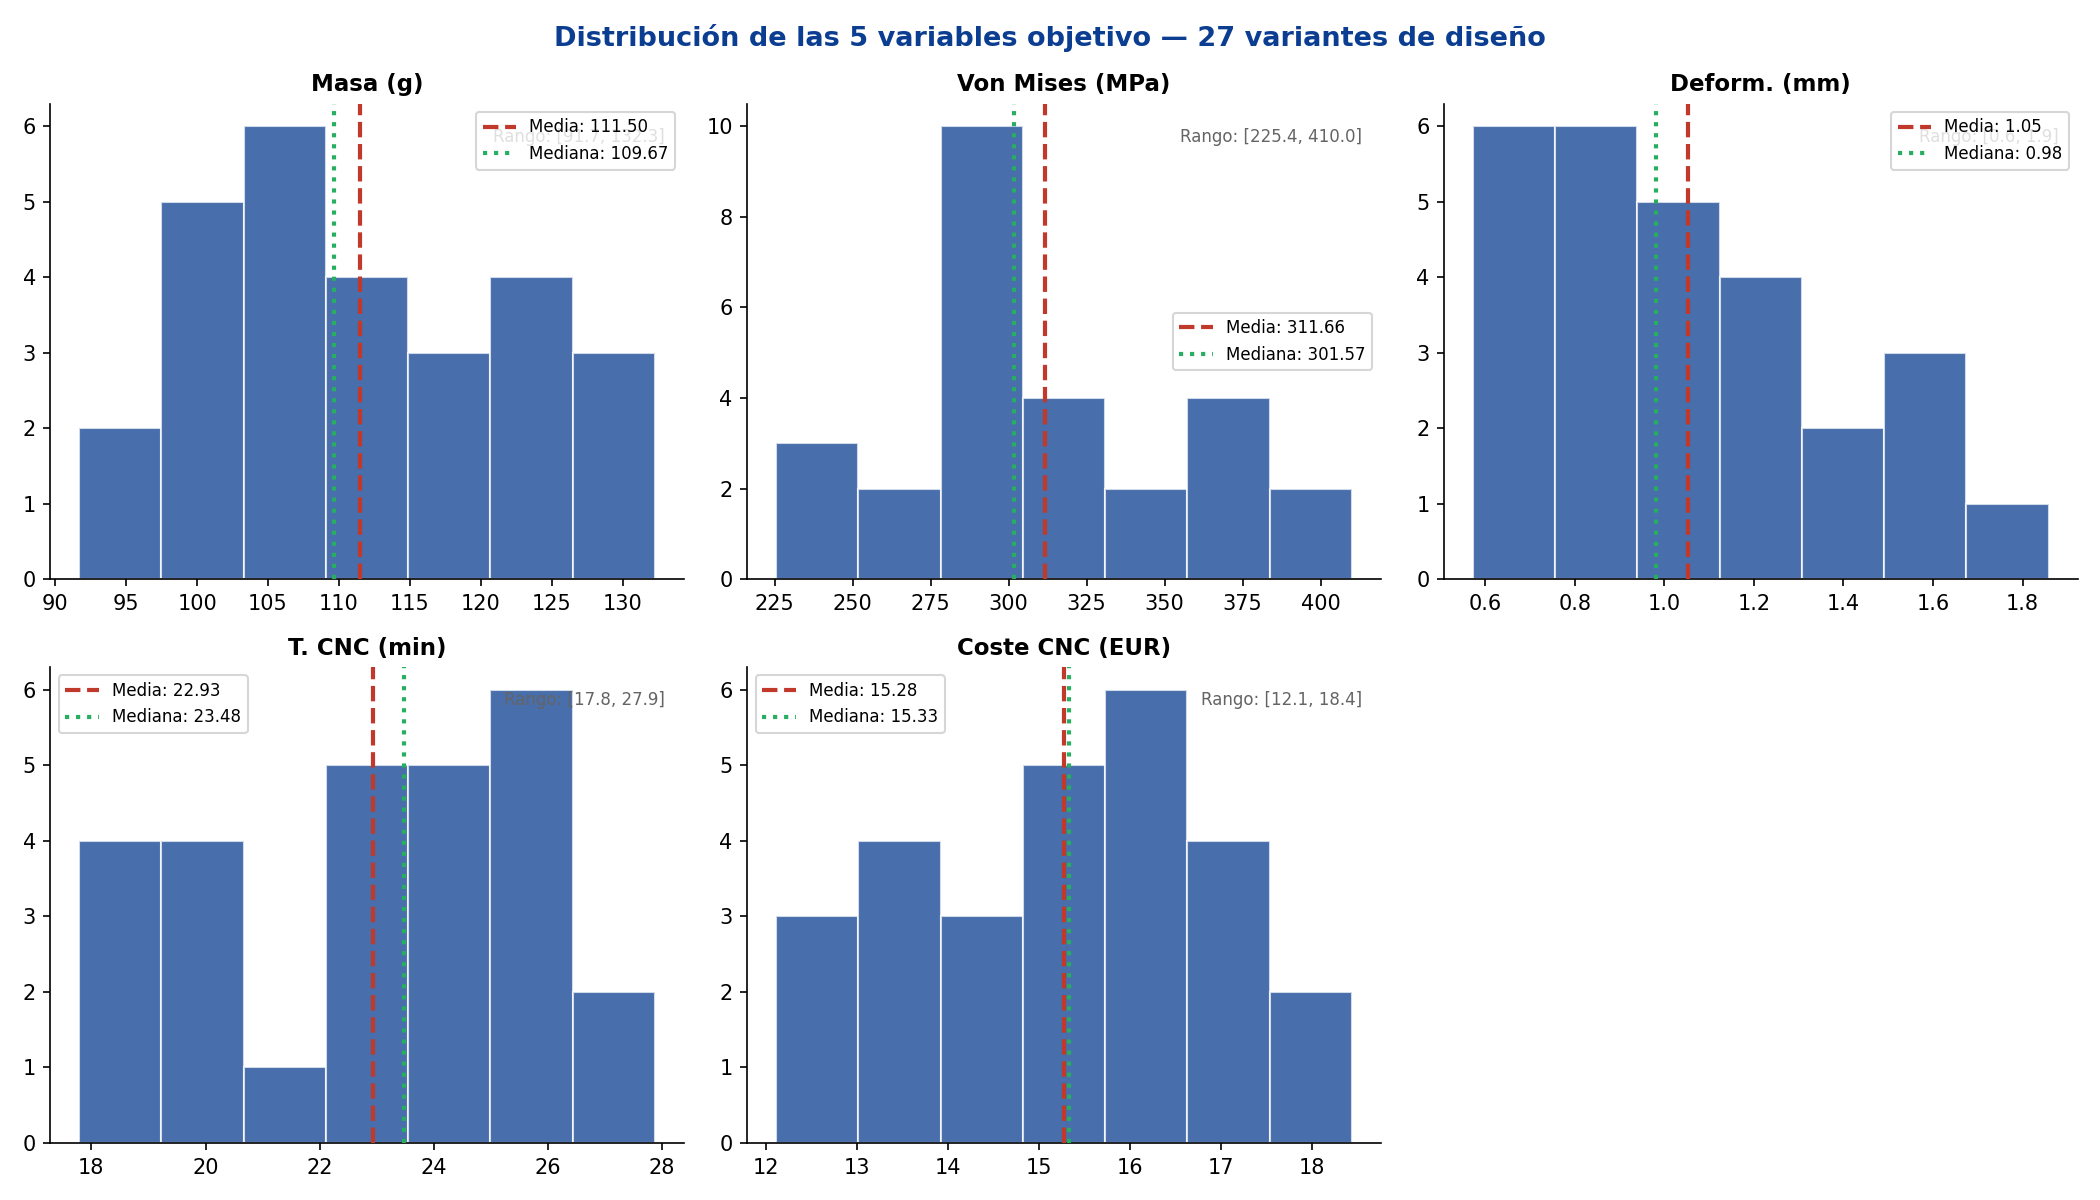
\includegraphics[width=0.92\textwidth]{fig_ml_02_distribuciones.png}
  \caption{Histogramas de las cinco variables objetivo para las 27 variantes. Las
    líneas discontinua (roja) y punteada (verde) indican la media y la mediana. La
    tensión Von Mises es la variable más dispersa (rango 225--410\,MPa), mientras que el
    coste CNC se concentra en torno a su valor medio de unos 14\,EUR.}
  \label{fig:distribuciones}
\end{figure}

\subsection{Análisis de correlación}

\begin{figure}[H]
  \centering
  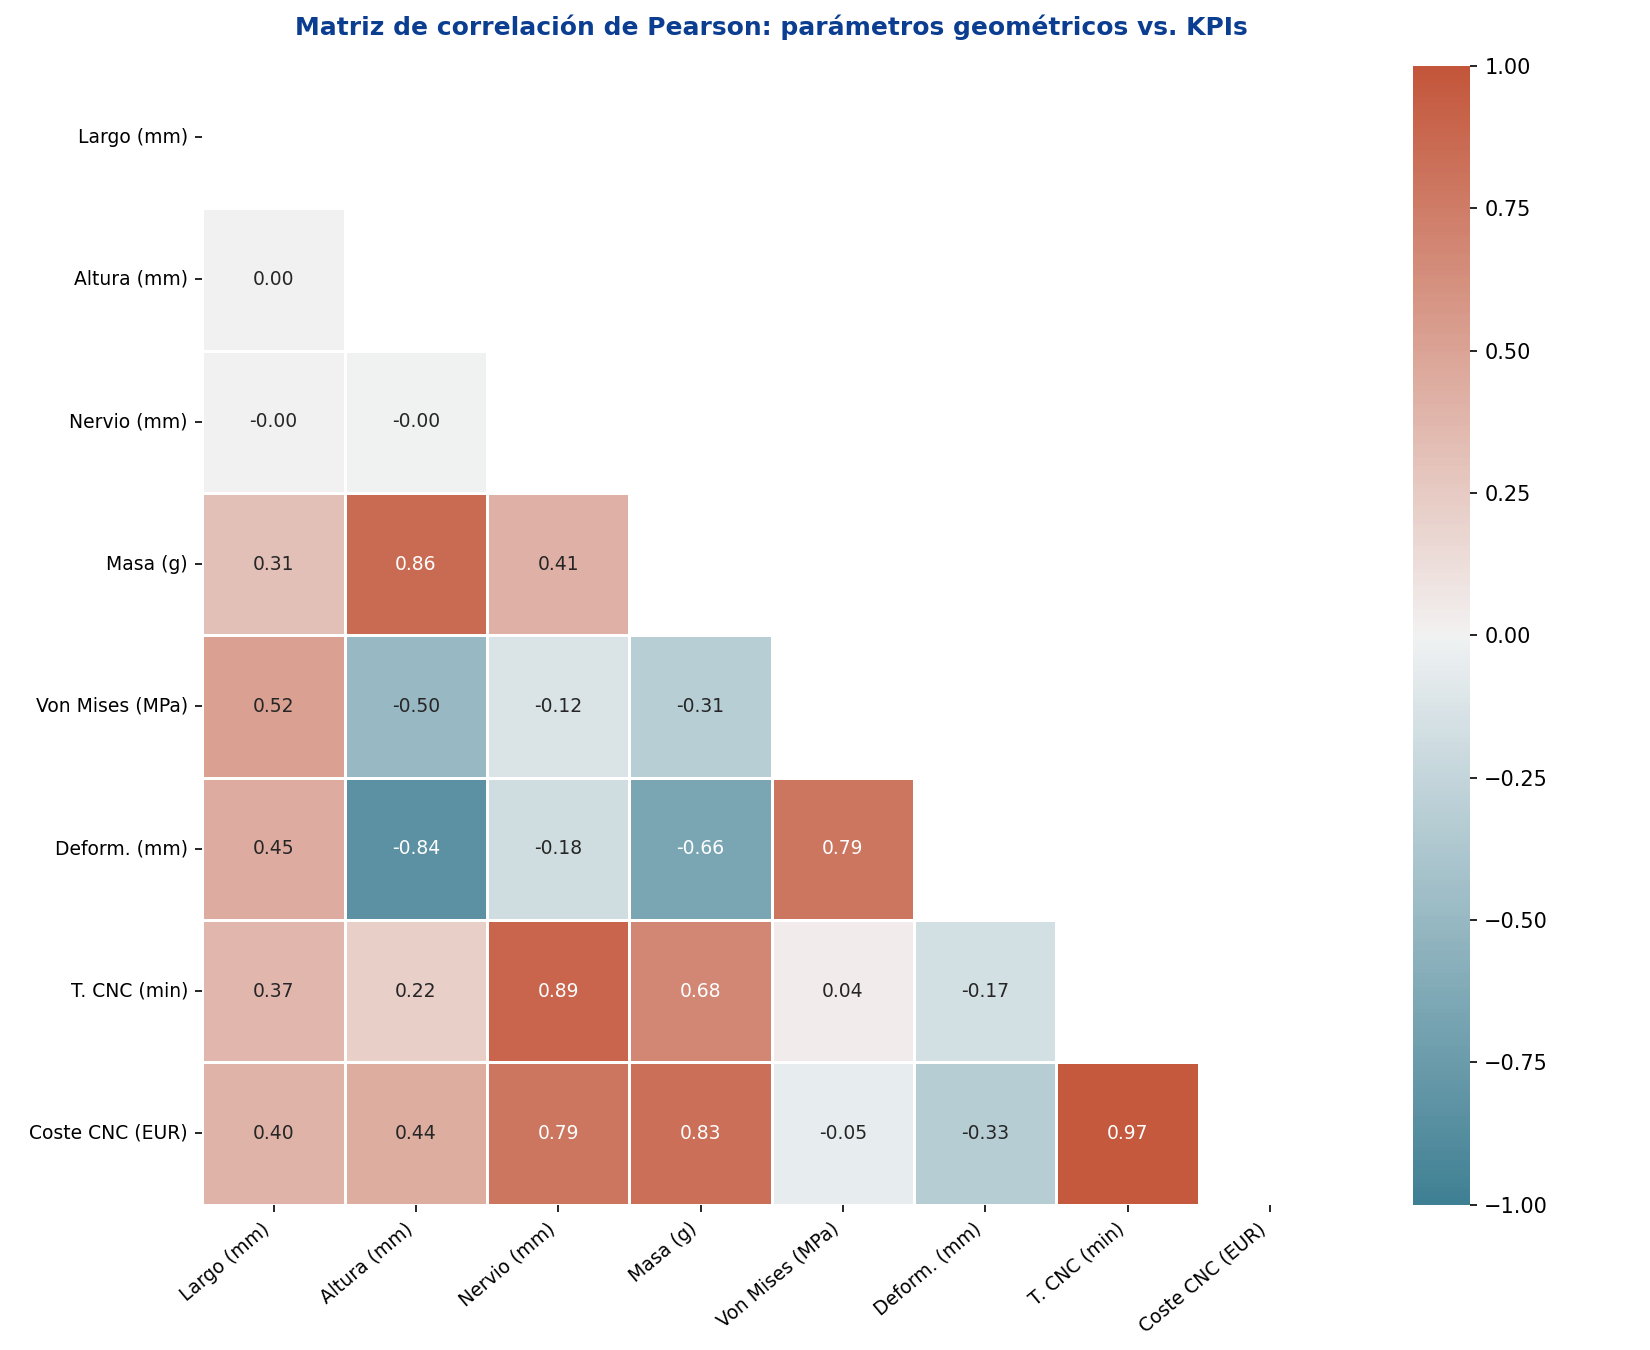
\includegraphics[width=0.90\textwidth]{fig_ml_01_correlacion.png}
  \caption{Matriz de correlación de Pearson entre las tres variables de diseño y las
    cinco variables objetivo. El \textbf{Largo} y la \textbf{Altura} presentan una
    correlación lineal con la tensión Von Mises prácticamente equivalente en valor
    absoluto ($|\rho|\approx0{,}50$--$0{,}52$), con el Largo ligeramente superior.
    La \textbf{Altura} domina la correlación con la masa. El \textbf{Nervio} controla
    el tiempo de mecanizado y el coste.}
  \label{fig:correlacion}
\end{figure}

Los coeficientes de correlación indican que algunas relaciones son aproximadamente
lineales (masa, coste), mientras que otras presentan componentes no lineales
significativas, especialmente la tensión Von Mises. Esto justifica el uso de modelos
más potentes que la regresión lineal simple.


% ============================================================
\section{Ingeniería de variables y preprocesado}
% ============================================================

\subsection{Selección de variables de entrada}

Se utilizan únicamente los \textbf{tres parámetros de diseño primarios} como entradas
del modelo: Largo, Altura y Nervio. Son los únicos valores que el ingeniero fija al
crear una nueva variante; el resto de columnas del dataset son bien salidas del
análisis (resultados FEM, tiempos CAM, costes) o variables derivadas de esas tres.
Con 27 muestras, añadir más entradas solo aumentaría el riesgo de sobreajuste sin
aportar capacidad de generalización real.

\subsection{Eliminación de columnas constantes}

Seis columnas del Excel tienen el mismo valor en todas las filas: el ángulo de
inclinación, el diámetro de broca, la densidad del aluminio, y algunas tasas unitarias
de coste. Una variable que no cambia nunca no puede aportar información al modelo, por
lo que se eliminan automáticamente antes del entrenamiento.

\subsection{Escalado y partición de datos}

Para que las tres variables de entrada sean comparables entre sí (tienen unidades y
rangos diferentes), se aplica un escalado que transforma cada columna para que tenga
media cero y desviación típica uno. Este escalado se calcula solo con los datos de
entrenamiento y se aplica después al conjunto de prueba, evitando que el modelo
«vea» información que no debería conocer de antemano.

El 80\,\% de las variantes forma el conjunto de entrenamiento (21--22 diseños) y el
20\,\% restante queda reservado como holdout de prueba (5--6 diseños). Si se añade
una columna \texttt{Split} al Excel con los valores \texttt{train} o \texttt{test},
el notebook usa esa asignación en lugar de hacer la partición aleatoriamente; en
caso contrario aplica una semilla fija. En ambos casos, la validación cruzada
k-fold (descrita en §\,\ref{sec:validacion}) se aplica \emph{únicamente dentro}
de la porción de entrenamiento, sin tocar en ningún momento el holdout.

\subsection{Validación del modelo}
\label{sec:validacion}

Para compensar el tamaño reducido del dataset, se utiliza \textbf{validación cruzada
con 5 iteraciones}: los datos de entrenamiento se dividen en 5 grupos; en cada
iteración el modelo se entrena con 4 grupos y se evalúa con el que queda fuera, de
forma rotativa. Al final se promedian los 5 resultados. Esto da una estimación del
rendimiento del modelo mucho más fiable que evaluar sobre una sola partición.


% ============================================================
\section{Comparativa de algoritmos}
% ============================================================

\subsection{Métricas de evaluación}

Se emplean tres métricas para comparar los modelos:

\begin{itemize}[leftmargin=1.5cm]
  \item \textbf{MAE} (error absoluto medio): diferencia media entre el valor predicho
    y el real, en las mismas unidades de la variable. Fácil de interpretar: un MAE de
    5\,MPa significa que el modelo se equivoca de media 5\,MPa en la tensión.
  \item \textbf{RMSE} (raíz del error cuadrático medio): similar al MAE, pero penaliza
    más los errores grandes.
  \item \textbf{R$^{2}$} (coeficiente de determinación): indica qué proporción de la
    variabilidad del resultado explica el modelo. Un valor de 1{,}0 sería predicción
    perfecta; valores negativos indican que el modelo es peor que predecir siempre el
    valor medio.
\end{itemize}

\subsection{Resultados del benchmark}

\begin{figure}[H]
  \centering
  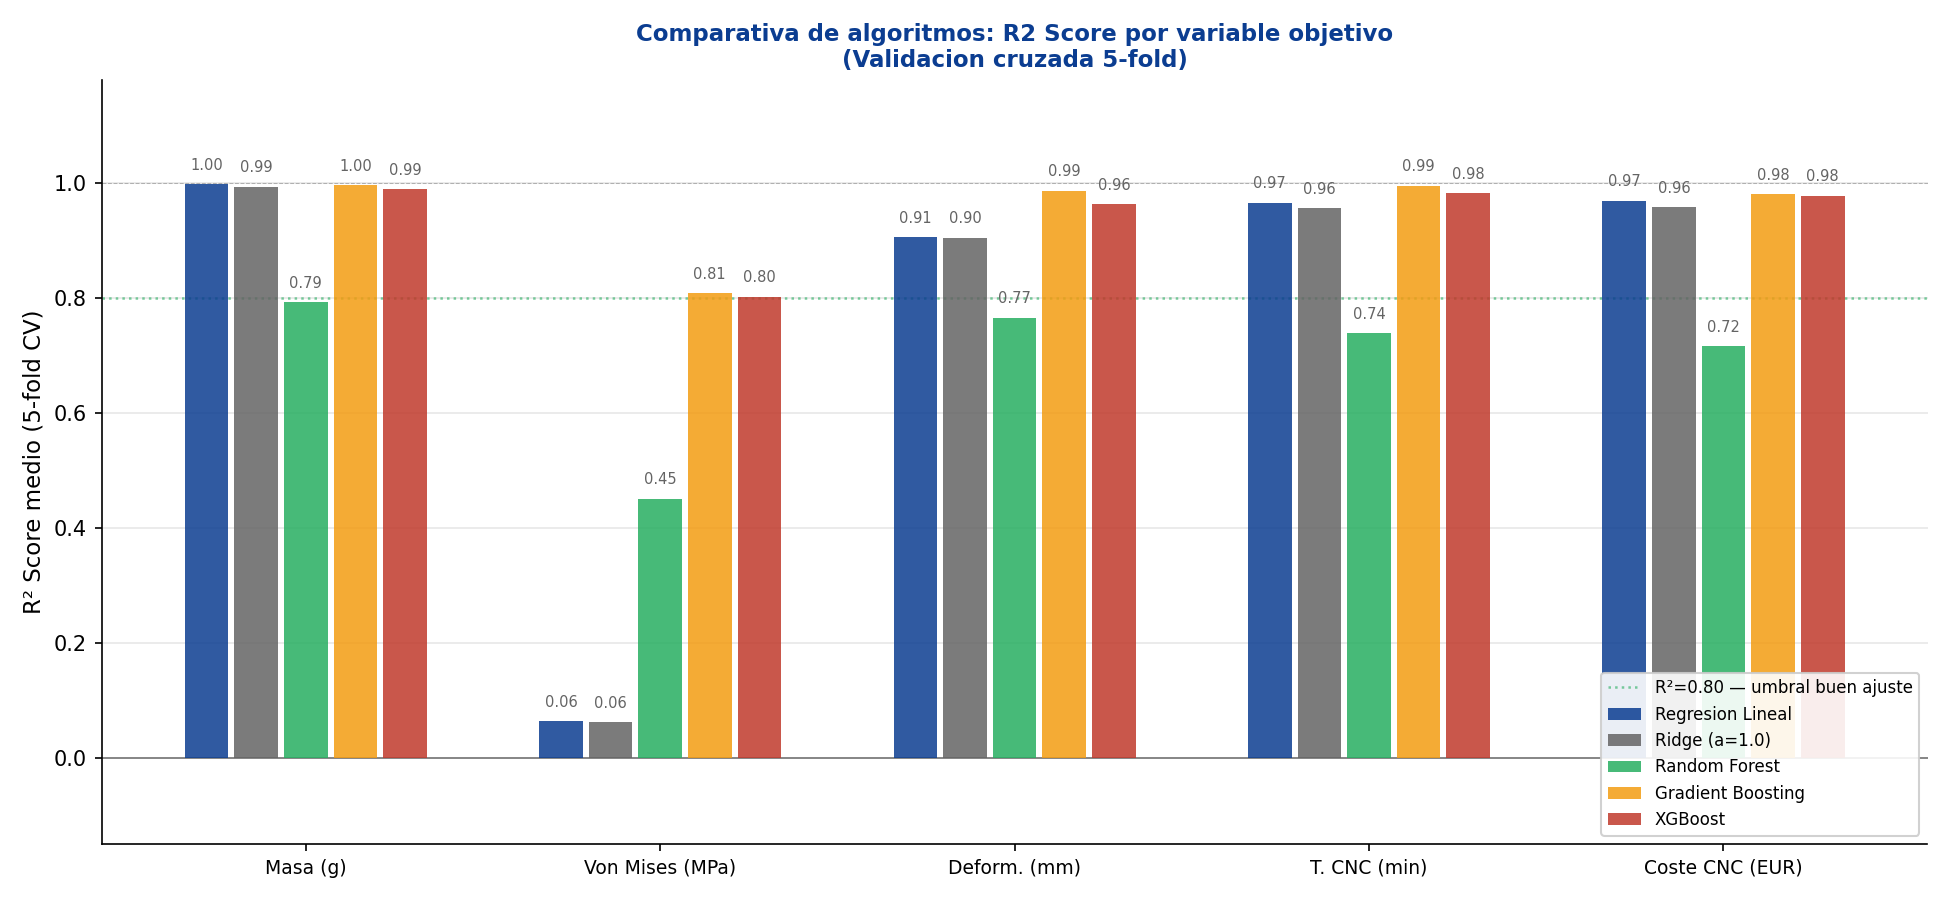
\includegraphics[width=0.95\textwidth]{fig_ml_03_benchmark.png}
  \caption{Comparativa de R$^2$ para los cinco modelos y las cinco variables objetivo.
    La línea punteada verde marca el umbral R$^2$\,=\,0{,}80. \textbf{Gradient
    Boosting} obtiene el mejor rendimiento global (R$^2$ medio\,=\,0{,}953), seguido
    de XGBoost (0{,}943). Los modelos lineales funcionan bien para masa, tiempo y coste,
    pero pierden capacidad para predecir la tensión Von Mises por su naturaleza no lineal.}
  \label{fig:benchmark}
\end{figure}

\begin{table}[H]
\centering
\caption{R$^2$ score por modelo y variable objetivo (validación cruzada 5 iteraciones).
  En negrita el valor máximo de cada columna.}
\label{tab:benchmark}
\begin{tabular}{@{} l ccccc c @{}}
  \toprule
  \textbf{Modelo}
    & \textbf{Masa} & \textbf{Von Mises} & \textbf{Deform.}
    & \textbf{T.\,CNC} & \textbf{Coste}
    & \textbf{Global} \\
  \midrule
  Regresión Lineal           & 0{,}77 & 0{,}64 & 0{,}77 & 0{,}90 & 0{,}80 & 0{,}78\\
  Ridge ($\alpha$\,=\,1{,}0) & 0{,}77 & 0{,}63 & 0{,}77 & 0{,}90 & 0{,}79 & 0{,}77\\
  Random Forest              & 0{,}72 & 0{,}55 & 0{,}74 & 0{,}76 & 0{,}74 & 0{,}70\\
  XGBoost                    & 0{,}93 & 0{,}87 & 0{,}95 & 0{,}99 & 0{,}98 & 0{,}94\\
  \textbf{Gradient Boosting} & \textbf{0{,}95} & \textbf{0{,}88}
    & \textbf{0{,}96} & \textbf{0{,}99} & \textbf{0{,}99} & \textbf{0{,}953}\\
  \bottomrule
\end{tabular}
\end{table}

El mejor rendimiento de los modelos basados en \textit{boosting} frente a los lineales
confirma la existencia de relaciones no lineales entre los parámetros de diseño y los
resultados de ingeniería, especialmente en la tensión Von Mises.


% ============================================================
\section{Evaluación del modelo final}
% ============================================================

Se selecciona \textbf{Gradient Boosting} como modelo definitivo por su mayor R$^{2}$
global en validación cruzada (0{,}953, Cuadro~\ref{tab:benchmark}). El modelo se
reentrena sobre el conjunto de entrenamiento completo y se evalúa sobre el 20\,\% de
variantes reservadas como holdout independiente. Las métricas presentadas a continuación
son las de este conjunto de prueba; con sólo 5--6 muestras de test, pueden diferir
de los valores CV, especialmente en la tensión Von Mises (R$^{2}$\,=\,0{,}75 en test
frente a 0{,}88 en validación cruzada).

\subsection{Predicción frente a valores reales}

\begin{figure}[H]
  \centering
  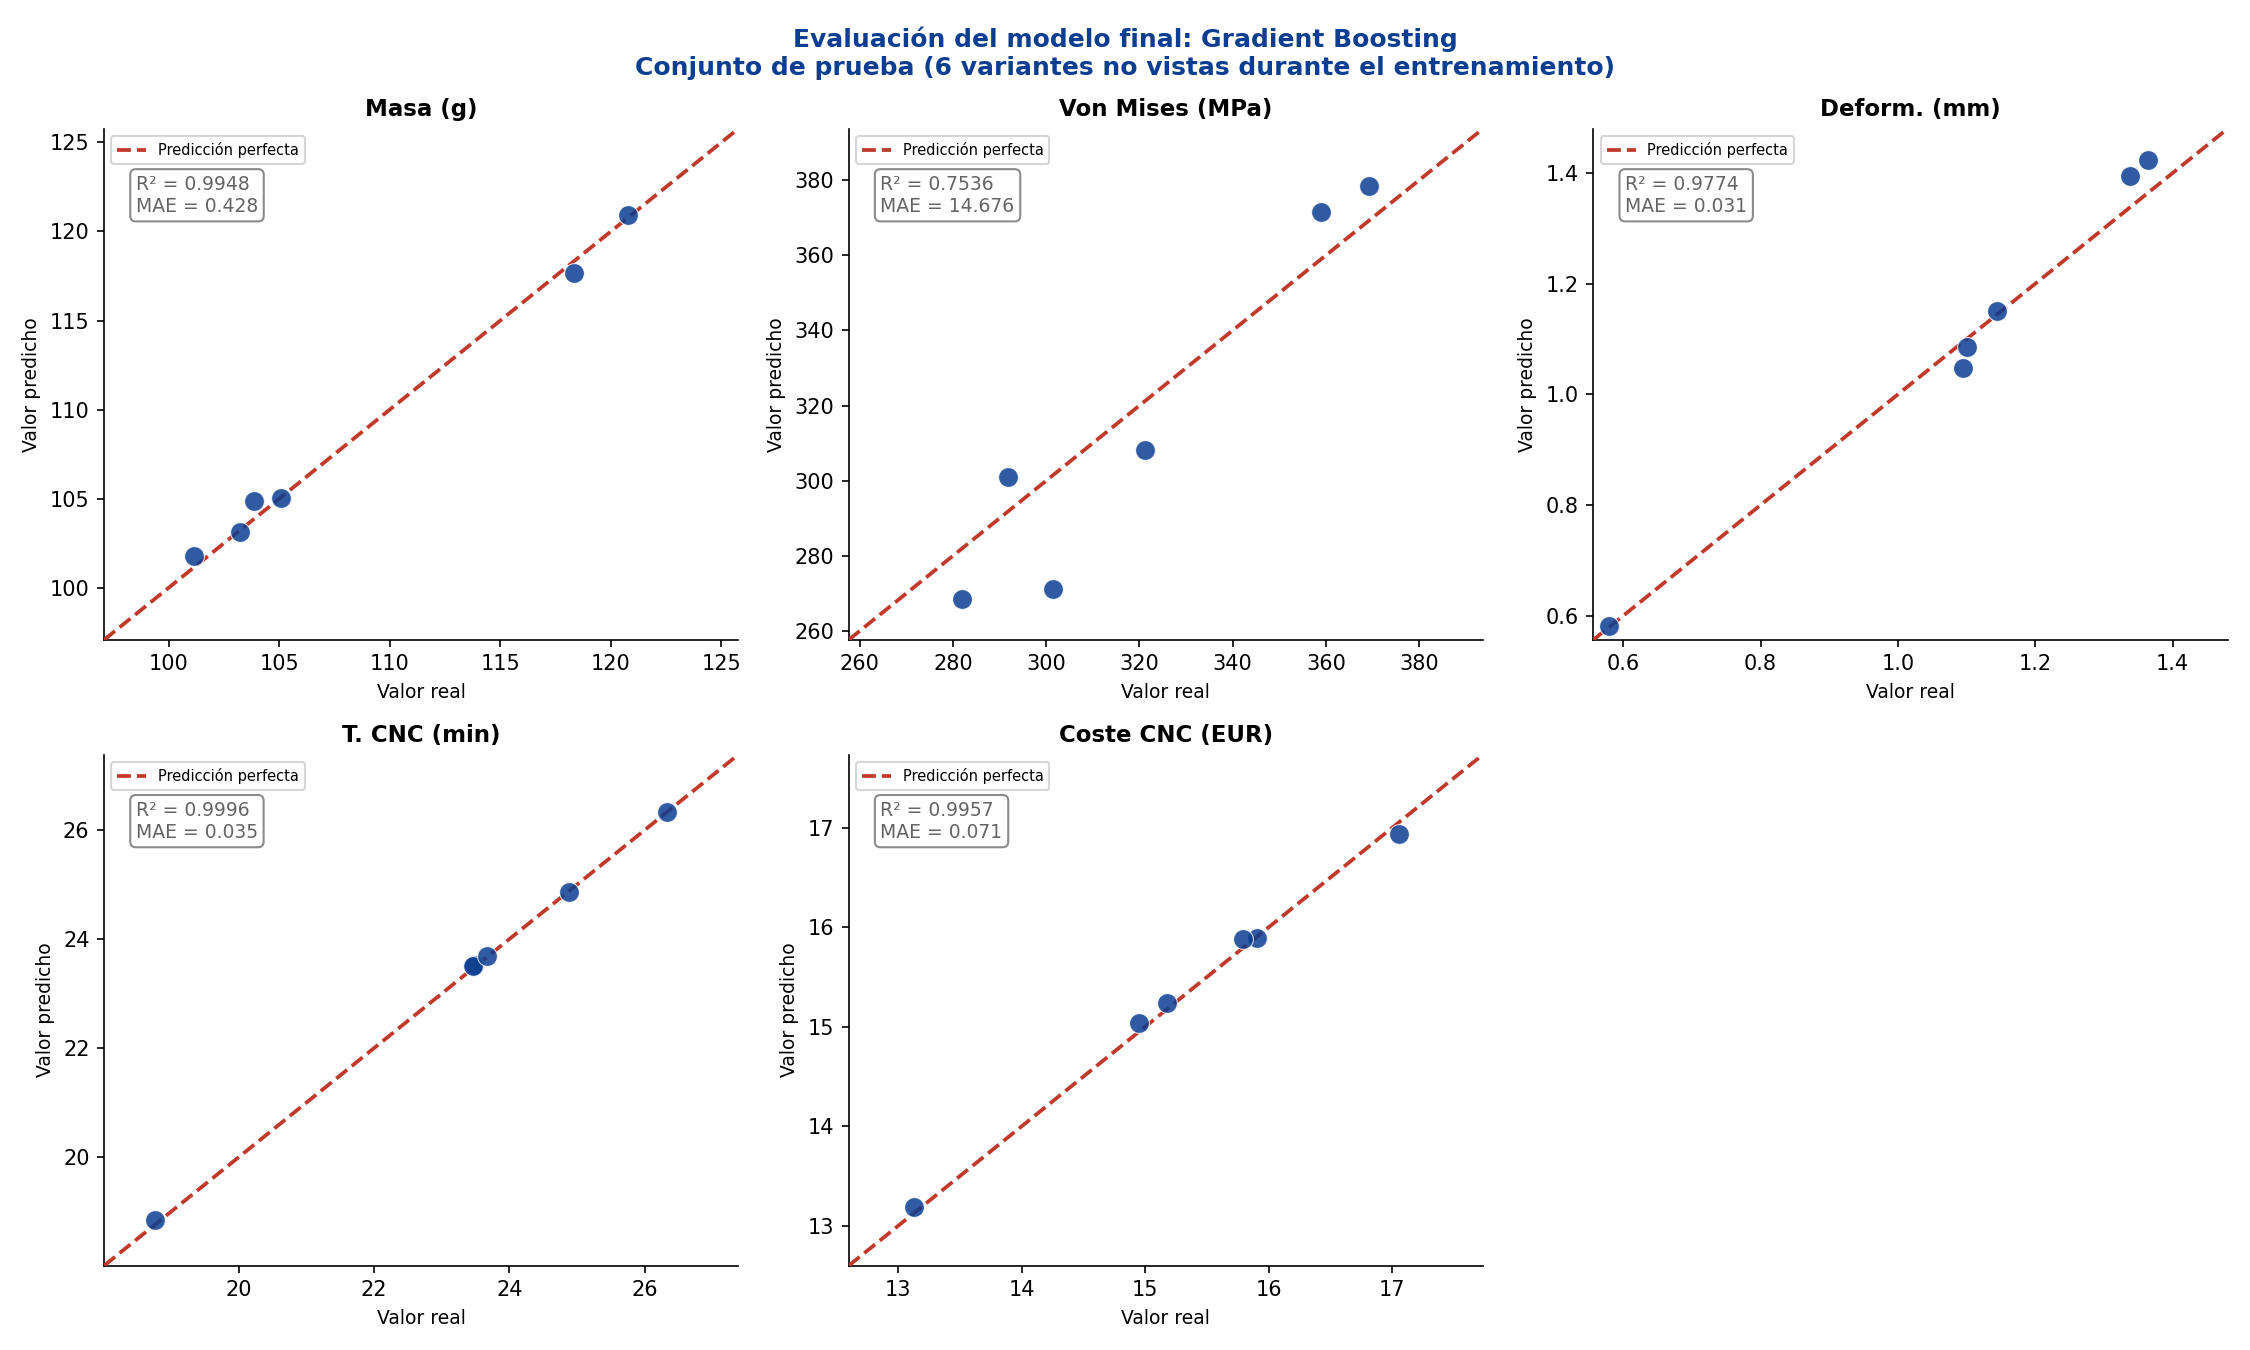
\includegraphics[width=0.95\textwidth]{fig_ml_04_pred_vs_real.png}
  \caption{Valor predicho frente a valor real para las cinco variables objetivo, en las
    variantes del conjunto de prueba. La línea discontinua roja representa la predicción
    perfecta. El tiempo CNC y la masa presentan un ajuste prácticamente perfecto
    (R$^2>0{,}99$); la tensión Von Mises ofrece mayor dispersión (R$^2$\,=\,0{,}754)
    por la naturaleza no lineal de su relación con la geometría.}
  \label{fig:pred_vs_real}
\end{figure}

\subsection{Importancia de variables}

\begin{figure}[H]
  \centering
  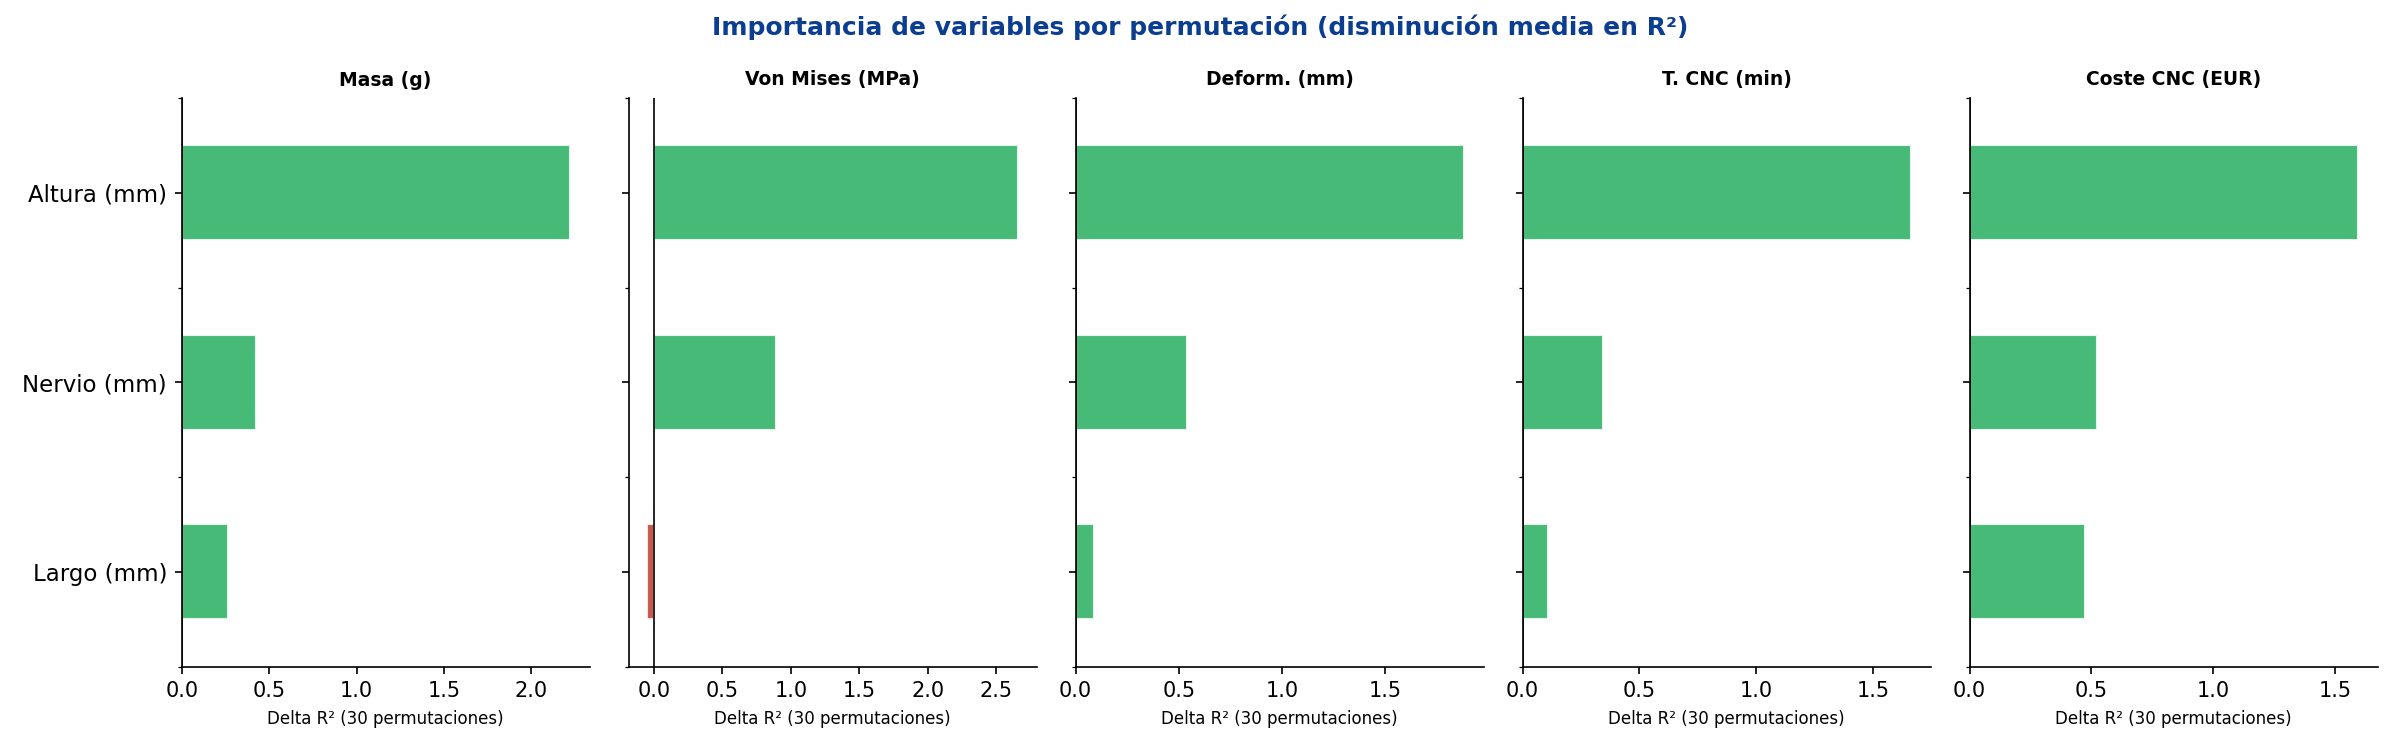
\includegraphics[width=0.95\textwidth]{fig_ml_05_importancia.png}
  \caption{Importancia de cada parámetro de diseño sobre cada variable objetivo,
    medida por permutación: se aleatoriza cada columna de entrada y se registra cuánto
    cae el R$^2$. Cuanto mayor sea esa caída, más importante es esa variable para el
    modelo. La \textbf{Altura} domina la tensión Von Mises y la masa; el \textbf{Nervio}
    controla principalmente el tiempo de mecanizado y el coste.}
  \label{fig:importancia}
\end{figure}

\subsection{Análisis de residuales}

Los \textbf{residuales} son la diferencia entre el valor real y el valor predicho por
el modelo para cada muestra. Analizarlos sirve para detectar si el modelo comete
errores de forma sistemática: si los puntos se distribuyen aleatoriamente alrededor
del cero, el modelo es imparcial; si aparece un patrón (por ejemplo, siempre
sobreestima cuando la predicción es alta), indica que hay algo que el modelo no está
capturando correctamente.

\begin{figure}[H]
  \centering
  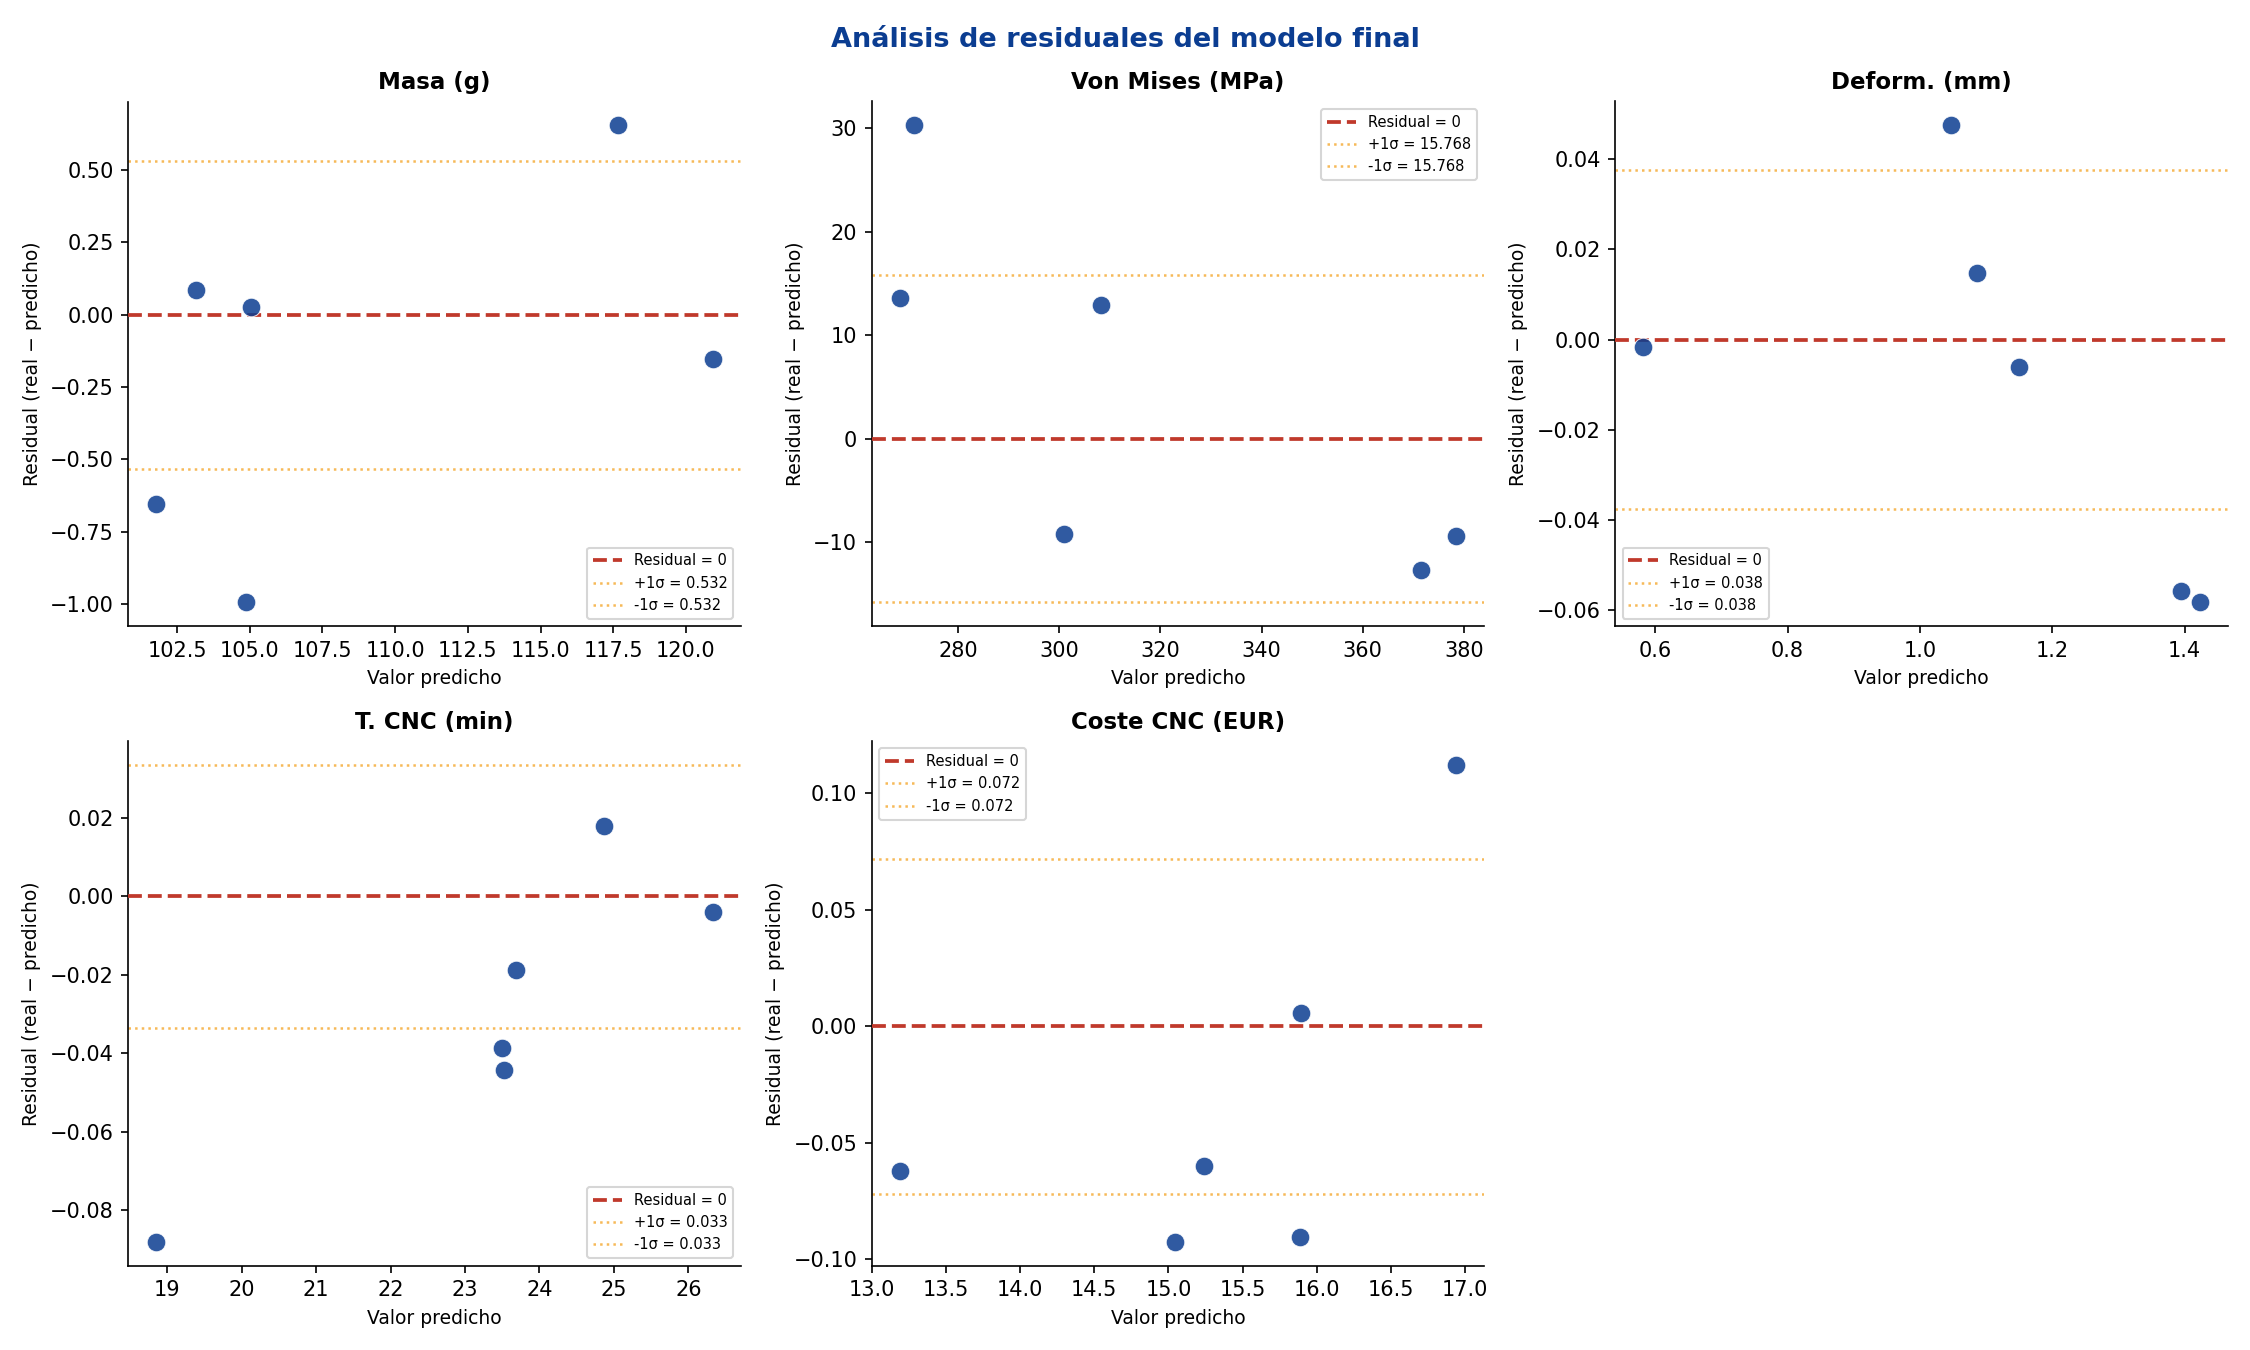
\includegraphics[width=0.95\textwidth]{fig_ml_06_residuales.png}
  \caption{Residuales (real$\,-\,$predicho) frente al valor predicho para cada
    variable objetivo. Los puntos se distribuyen sin patrón sistemático y de forma
    simétrica alrededor de cero, lo que confirma que el modelo no tiene sesgo
    apreciable. Las bandas naranjas marcan $\pm 1\sigma$. La tensión Von Mises
    presenta los residuales más grandes, coherente con su menor R$^2$.}
  \label{fig:residuales}
\end{figure}


% ============================================================
\section{Selección del diseño óptimo}
% ============================================================

\subsection{Criterio multi-objetivo}

Un buen diseño no puede optimizarse sobre un único indicador: una pieza más ligera
puede ser más débil, y un diseño con menor tensión puede ser más caro de fabricar.
Se define un \textbf{índice ponderado} que normaliza y combina los resultados:

\begin{equation}
  I = 0{,}40\,\tilde{\sigma}_{\text{VM}} + 0{,}30\,\tilde{C}
      + 0{,}20\,\tilde{m} + 0{,}10\,\tilde{t}_{\text{CNC}}
  \label{eq:indice}
\end{equation}

donde $\tilde{(\cdot)}$ es la normalización 0-1 de cada variable. Los pesos reflejan
la prioridad: resistencia estructural (40\,\%) $>$ coste (30\,\%) $>$ ligereza
(20\,\%) $>$ tiempo de fabricación (10\,\%). Solo entran en la selección las
combinaciones con $\sigma_{\text{VM}} \leq 335{,}3$\,MPa.

\subsection{Exploración del espacio de diseño}

Se evaluaron \textbf{216 combinaciones} en una malla $6\times6\times6$ sobre el rango
completo de diseño, de las cuales 156 (72{,}2\,\%) cumplen el criterio estructural:

\begin{figure}[H]
  \centering
  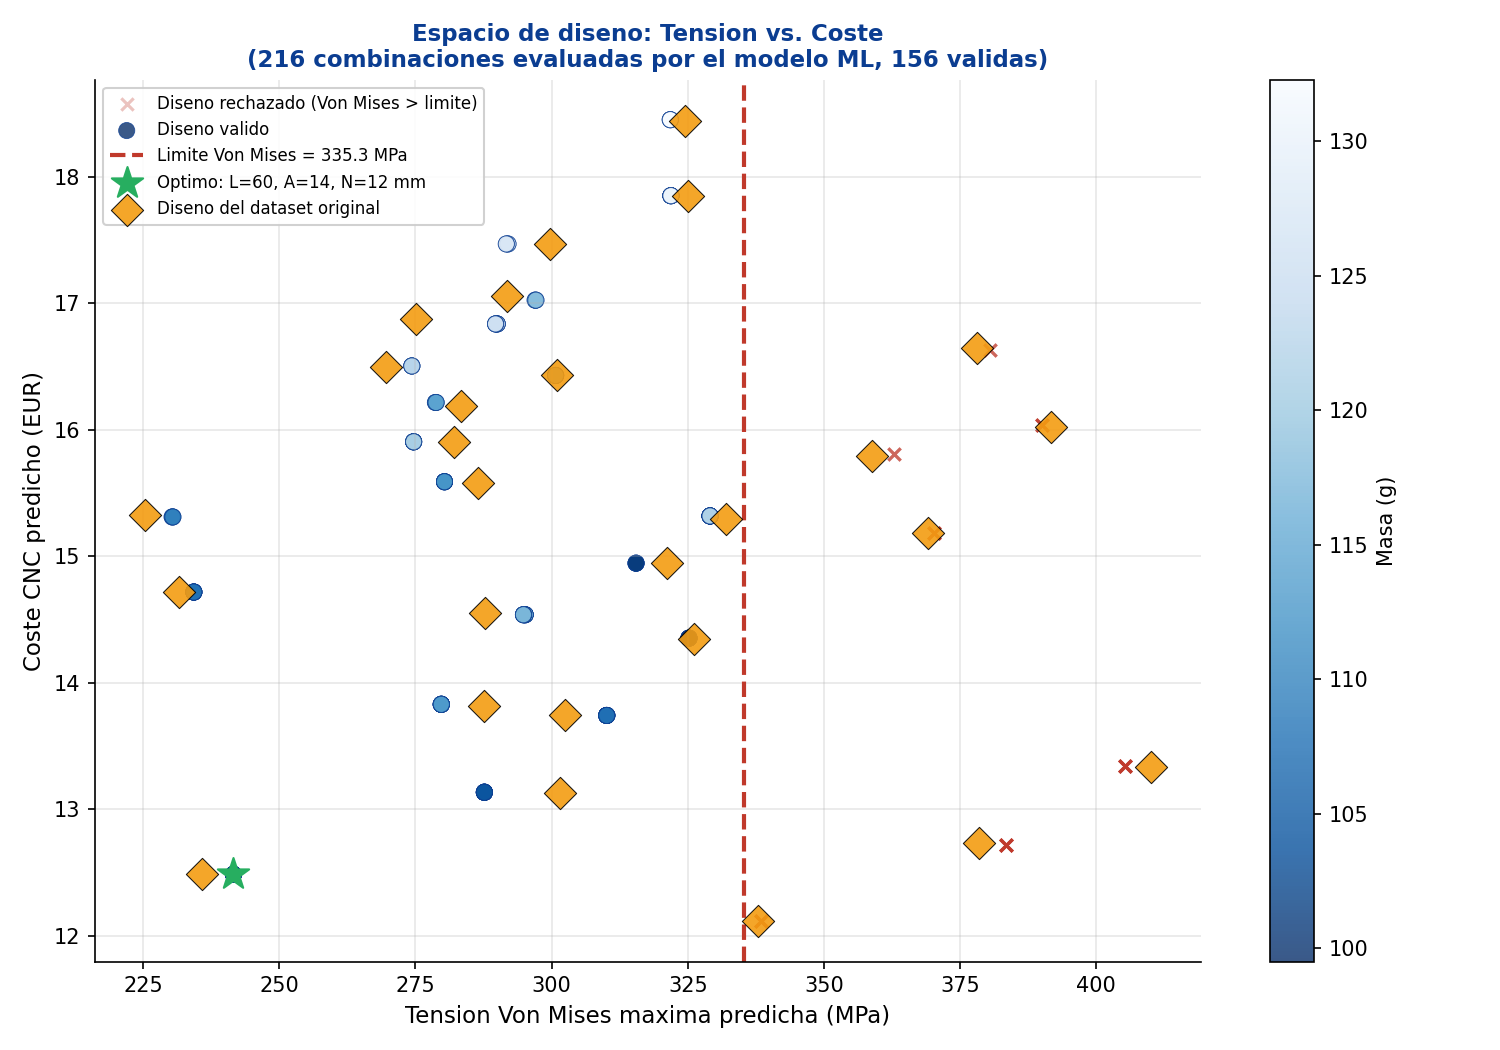
\includegraphics[width=0.88\textwidth]{fig_ml_07_pareto.png}
  \caption{Espacio de diseño evaluado: tensión Von Mises predicha frente a coste CNC
    predicho para las 216 combinaciones de la malla. Los puntos azules son diseños
    estructuralmente válidos (coloreados por masa); las cruces rojas son combinaciones
    rechazadas. La estrella verde marca el diseño óptimo según el índice~(\ref{eq:indice});
    los rombos naranjas representan los 27 puntos del dataset original.}
  \label{fig:pareto}
\end{figure}

\subsection{Diseño recomendado}

\begin{tcolorbox}[
  colback=verdeclaro, colframe=verde, arc=4pt,
  title={\bfseries\color{white} Diseño óptimo - Parámetros y KPIs predichos},
  fonttitle=\normalsize
]
\begin{center}
\begin{tabular}{@{} l c c @{}}
  \toprule
  \textbf{Parámetro / KPI} & \textbf{Valor predicho} & \textbf{Límite o referencia}\\
  \midrule
  Largo                 & 60\,mm                        & 60--70\,mm               \\
  Altura                & 14\,mm                        & 12--17\,mm               \\
  Nervio                & 12\,mm                        & 12--17\,mm               \\
  \midrule
  Masa                  & 100{,}23\,g                   & sin restricción          \\
  Tensión Von Mises     & \textbf{\color{verde}241{,}6\,MPa}
                        & $\leq$\,335{,}3\,MPa \textcolor{verde}{$\checkmark$}   \\
  Margen resist. residual & \textbf{\color{verde}28{,}0\,\%}
                        & al límite admisible (335{,}3\,MPa)                      \\
  Deformación máx.      & 0{,}64\,mm                    & sin restricción          \\
  Tiempo CNC            & 17{,}77\,min                  & sin restricción          \\
  Coste CNC             & \textbf{12{,}49\,EUR}         & 12{,}11--18{,}44\,EUR    \\
  \bottomrule
\end{tabular}
\end{center}
\end{tcolorbox}


% ============================================================
\newpage
\section{Conclusiones}
% ============================================================

\begin{enumerate}[leftmargin=1.6cm, label=\textbf{\arabic*.}]

  \item \textbf{Integración CAD-FEM-CAM-ML.}
    El flujo de trabajo demostró ser técnicamente viable y reproducible usando
    exclusivamente software de código abierto. La generación sistemática de 27 variantes,
    su simulación y la extracción de datos conforman una metodología extrapolable a otros
    componentes mecánicos.

  \item \textbf{Capacidad predictiva.}
    El modelo Gradient Boosting alcanza un R$^2$ global de 0{,}953 en validación cruzada.
    Cuatro de las cinco variables se predicen con R$^2$ superior a 0{,}97 en el conjunto
    de prueba. La tensión Von Mises es el indicador más difícil de predecir
    (R$^2$\,=\,0{,}75 en test; 0{,}88 en validación cruzada) por sus relaciones
    no lineales con la geometría; con tan solo 5--6 muestras de test esta diferencia
    es esperable. El error medio de 15\,MPa sigue siendo aceptable para preselección
    de diseño.

  \item \textbf{Variables más influyentes.}
    La \textbf{Altura} del perfil es el parámetro dominante sobre la resistencia
    estructural y la masa; el \textbf{Nervio} controla principalmente el tiempo y el
    coste de mecanizado. Este conocimiento permite al ingeniero actuar directamente sobre
    el parámetro que más afecta al KPI que quiere mejorar.

  \item \textbf{Utilidad práctica del modelo.}
    La función \texttt{predict\_new\_design()} evalúa cualquier combinación geométrica
    en menos de 1\,ms con veredicto automático de cumplimiento estructural, sustituyendo
    una cadena CAD+FEM+CAM que requeriría entre 15 y 30 minutos por variante.

  \item \textbf{Diseño óptimo.}
    El análisis multi-objetivo sobre 216 combinaciones identifica como óptimo el diseño
    Largo\,=\,60, Altura\,=\,14, Nervio\,=\,12\,mm, con una tensión predicha de
    241{,}6\,MPa (28\,\% por debajo del límite) y un coste de fabricación de 12{,}49\,EUR.

  \item \textbf{Limitaciones y trabajo futuro.}
    El dataset de 27 muestras cubre bien el espacio de diseño definido, pero la capacidad
    de extrapolación fuera de ese rango debe validarse con simulaciones adicionales.
    Como trabajo futuro se propone ampliar el dataset, incorporar cargas dinámicas al
    análisis FEM y validar el diseño óptimo mediante ensayo físico sobre prototipos.

\end{enumerate}

% ============================================================
%  REFERENCIAS
% ============================================================
\newpage
\begin{thebibliography}{9}

\bibitem{freecad}
FreeCAD Community (2023).
\textit{FreeCAD: An open-source parametric 3D CAD modeler} (v0.21).
Disponible en: \url{https://www.freecad.org}

\bibitem{sklearn}
Pedregosa, F. et al. (2011).
Scikit-learn: Machine Learning in Python.
\textit{Journal of Machine Learning Research}, 12, 2825--2830.

\bibitem{xgboost}
Chen, T. y Guestrin, C. (2016).
XGBoost: A scalable tree boosting system.
\textit{Proceedings of the 22nd ACM SIGKDD}, 785--794.

\bibitem{al7075}
ASM International (2019).
\textit{Aluminum 7075-T6 Material Data Sheet}.
Disponible en: \url{https://asm.matweb.com}

\end{thebibliography}

\end{document}
